%%%%%%%%%%%%%%%%%%%%%%%%%%%%%%%%%%%%%%%%%%%%%%%%%%%%%%%%%%%%%%%%%%%%%%%%%%%%%%%%%%%%%%%%%%%%%%%%%%%%%%
% Plantilla básica de Latex en Español.
%
% Autor: Andrés Herrera Poyatos (https://github.com/andreshp) 
%
% Es una plantilla básica para redactar documentos. Utiliza el paquete fancyhdr para darle un
% estilo moderno pero serio.
%
% La plantilla se encuentra adaptada al español.
%
%%%%%%%%%%%%%%%%%%%%%%%%%%%%%%%%%%%%%%%%%%%%%%%%%%%%%%%%%%%%%%%%%%%%%%%%%%%%%%%%%%%%%%%%%%%%%%%%%%%%%%

%-----------------------------------------------------------------------------------------------------
%	INCLUSIÓN DE PAQUETES BÁSICOS
%-----------------------------------------------------------------------------------------------------

\documentclass[10pt]{article}

%-----------------------------------------------------------------------------------------------------
%	SELECCIÓN DEL LENGUAJE
%-----------------------------------------------------------------------------------------------------

% Paquetes para adaptar Látex al Español:
\usepackage[spanish,es-noquoting, es-tabla, es-lcroman]{babel} % Cambia 
\usepackage[utf8]{inputenc}                                    % Permite los acentos.
\selectlanguage{spanish}                                       % Selecciono como lenguaje el Español.

%-----------------------------------------------------------------------------------------------------
%	SELECCIÓN DE LA FUENTE
%-----------------------------------------------------------------------------------------------------

% Fuente utilizada.
\usepackage{microtype}                  % Mejora la letra final de cara al lector.
\usepackage{helvet}

\renewcommand{\familydefault}{\sfdefault}

%-----------------------------------------------------------------------------------------------------
%	ESTILO DE PÁGINA
%-----------------------------------------------------------------------------------------------------

% Paquetes para el diseño de página:
\usepackage{fancyhdr}               % Utilizado para hacer títulos propios.
\usepackage{lastpage}               % Referencia a la última página. Utilizado para el pie de página.
\usepackage{extramarks}             % Marcas extras. Utilizado en pie de página y cabecera.
\usepackage[parfill]{parskip}       % Crea una nueva línea entre párrafos.
\usepackage{geometry}               % Asigna la "geometría" de las páginas.

% Se elige el estilo fancy y márgenes de 3 centímetros.
\pagestyle{fancy}
\geometry{left=3cm,right=3cm,top=2.5cm,bottom=2.5cm,headheight=1cm,headsep=0.5cm} % Márgenes y cabecera.
% Se limpia la cabecera y el pie de página para poder rehacerlos luego.
\fancyhf{}

% Espacios en el documento:
\linespread{1}                        % Espacio entre líneas.
\setlength\parindent{0pt}               % Selecciona la indentación para cada inicio de párrafo.

% Cabecera del documento. Se ajusta la línea de la cabecera.
\renewcommand\headrule{
	\begin{minipage}{1\textwidth}
	    \hrule width \hsize 
	\end{minipage}
}

% Texto de la cabecera:
\lhead{\subject}               % Parte izquierda.
\chead{}                       % Centro.
\rhead{\doctitle}              % Parte derecha.

% Pie de página del documento. Se ajusta la línea del pie de página.
\renewcommand\footrule{                                 
\begin{minipage}{1\textwidth}
    \hrule width \hsize   
\end{minipage}\par
}

\lfoot{}                                                 % Parte izquierda.
\cfoot{}                                                 % Centro.
\rfoot{Página\ \thepage\ de\ \protect\pageref{LastPage}} % Parte derecha.

%-----------------------------------------------------------------------------------------------------
%	IMÁGENES
%-----------------------------------------------------------------------------------------------------

\usepackage{graphicx}                  % Utilizado para insertar gráficos.
\usepackage{caption}                   % Títulos y leyendas para los gráficos.
\usepackage{subcaption}                % Subfiguras.
\usepackage{float}

%-----------------------------------------------------------------------------------------------------
%	BIBLIOGRAFÍA
%-----------------------------------------------------------------------------------------------------

\usepackage[backend=bibtex]{biblatex}
\usepackage{csquotes}

\addbibresource{references.bib}

%-----------------------------------------------------------------------------------------------------
%	ALGORITMOS
%-----------------------------------------------------------------------------------------------------

\usepackage{algorithm}
\usepackage{algpseudocode}
\usepackage{subcaption}
\captionsetup{compatibility=false}
\DeclareCaptionSubType*{algorithm}
\renewcommand\thesubalgorithm{\thetable\alph{subalgorithm}}
\DeclareCaptionLabelFormat{alglabel}{Alg.~#2}

%-----------------------------------------------------------------------------------------------------
%	PORTADA
%-----------------------------------------------------------------------------------------------------

% Elija uno de los siguientes formatos.
% No olvide incluir los archivos .sty asociados en el directorio del documento.
%\usepackage{title1}
%\usepackage{title2}
%\usepackage{title3}

% Primera letra más grande
\usepackage{lettrine}

% Primera página diferente
\fancypagestyle{plain}
{
	\fancyhf{}
	\renewcommand{\headrule}{}
	\rfoot{Página\ \thepage\ de\ \protect\pageref{LastPage}}
}

%-----------------------------------------------------------------------------------------------------
%	TÍTULO, AUTOR Y OTROS DATOS DEL DOCUMENTO
%-----------------------------------------------------------------------------------------------------

% Título del documento.
\newcommand{\doctitle}{Big Data, Map Reduce y TPCx-HS}
% Subtítulo.0
\newcommand{\docsubtitle}{}
% Fecha.
\newcommand{\docdate}{28 \ de \ Marzo \ de \ 2015}
% Asignatura.
\newcommand{\subject}{Ingeniería de Servidores}
% Autor.
\newcommand{\docauthor}{}
\newcommand{\docaddress}{}
\newcommand{\docemail}{}

%-----------------------------------------------------------------------------------------------------
%	RESUMEN
%-----------------------------------------------------------------------------------------------------

% Resumen del documento. Va en la portada.
% Puedes también dejarlo vacío, en cuyo caso no aparece en la portada.
%\newcommand{\docabstract}{}
\newcommand{\docabstract}{
	\setlength\parindent{0pt}
	
	El término Big Data se ha vuelto muy popular, pudiendo encontrarlo a menudo en múltiples noticias de la prensa tecnológica. Estas noticias destacan principalmente dos aspectos de Big Data: la gran cantidad de datos a analizar y las posibles aplicaciones. Sin embargo, las tecnologías subyacentes son menos conocidas.

	\kern2mm
	En este trabajo presentamos una introducción a Big Data destacando el papel que ejerce en este ámbito la ingeniería de servidores. En primer lugar, motivamos y definimos el concepto de Big Data, mostrando la necesidad de desarrollar nuevas tecnologías que permitan abordar problemas de este campo. El desarrollo de estas tecnologías se encuentra ligado a la ingeniería de servidores y a la computación de altas prestaciones. Posteriormente, explicamos map reduce, un nuevo paradigma de programación distribuida, y Hadoop, una de las tegnologías que implementa Map Reduce más importantes del estado del arte. Por último, introducimos TPCx-HS, un benchmark para computadores que utilicen Hadoop, y destacamos el trabajo que queda por hacer en este ámbito.}

	\providecommand{\keywords}[1]{\textbf{\textit{Palabras clave---}} #1
}

\begin{document}

\makeatletter\renewcommand{\ALG@name}{Algoritmo}

%\maketitle

\thispagestyle{plain}

\begin{center}
	\huge{\textbf{\doctitle}}	
\end{center}

\vspace*{0.5cm}

\noindent\fbox{
	\parbox{\textwidth}{
		\kern3mm
		\begin{abstract} 
			\docabstract
		\end{abstract}
		\vspace*{0.3cm}
		\centering\keywords{Big Data, Map Reduce, Hadoop, TPCx-HS, benchmarks, ingeniería de servidores}

		\kern3mm
	}
}

%-----------------------------------------------------------------------------------------------------
%	SECCIÓN 1: INTRODUCCIÓN
%-----------------------------------------------------------------------------------------------------

\section{Introducción} \label{sec:introduction}
	
	\lettrine[lraise=0.1, nindent=0em, slope=-.5em]{D}{}esde hace miles de años el ser humano ha investigado la manera de almacenar y recopilar información. Durante muchos siglos la escritura y la pintura eran los únicos mecanismos existentes. Posteriormente surgió la fotografía, los discos de vinilo... Sin embargo, poca información seguía ocupando mucho volumen físico. Gracias a los avances tecnológicos de las últimos décadas, hoy en día disponemos dispositivos electrónicos para el almacenamiento de datos binarios. Además, la evolución de estos dispositivos ha sido frenética. IBM comercializó el primer disco duro en 1956. Este constaba solamente de 5 mega bytes de capacidad \cite{hard-disks} mientras que actualmente podemos utilizar discos duros con más de 1 tera byte.

	La capacidad de cómputo y procesamiento de los computadores también ha crecido de forma exponencial. El primer ordenador comercial se presentó en 1951 y se conoce como  UNIVAC 1 \cite{first-commercial-computer}. Este computador tenía una frecuencia de $2.25$ mega hercios y $1000$ palabras de memoria principal o RAM \cite{caract}. Actualmente utilizamos procesadores con más de $2$ giga hercios de frecuencia de reloj. Además, es habitual encontrar computadores con $8$ o más giga bytes de memoria principal, lo que permite trabajar con bastante información de forma eficiente. 

	Estas nuevas tecnologías han posibilitado que el almacenamiento de datos sea mucho más sencillo. Podemos guardar multitud de archivos en un dispositivo de unos centímetros y compartirlos con cualquier usuario. Además, el procesamiento de estos archivos a nivel de usuario es eficiente gracias a la velocidad de los computadores. 
	
	El mayor flujo de datos es producido en Internet. Aunque es relativamente joven, se hizo público en 1993, actualmente existen más de mil millones de páginas webs \cite{internet}. Además, multitud de dispositivos electrónicos se conectan e interaccionan con Internet (lo que se denomina Internet de las cosas \cite{big-data-internet-cosas}). Los usuarios de estos dispositivos utilizan aplicaciones web y redes sociales, publicando textos y archivos multimedia. 
	
	Todo este cúmulo de tecnologías y actividades ha dado lugar a que hoy en día haya más de $10$ zeta bytes de información almacenados ($1$ ZB = $10^{12}$ GB). La Figura \ref{fig:zeta-bytes} muestra la evolución histórica de la cantidad de información acumulada por el ser humano. Podemos observar que cada año se generan varios zeta bytes de información, el crecimiento es exponencial. Hasta 2003 se habían almacenado en total $5$ exa bytes de información ($1$ EB = $10^9$ GB). Actualmente, generamos esta cantidad de datos en dos días \cite{big-data}. Por tanto, podemos concluir que vivimos en una sociedad digital o sociedad de la información.

	\begin{figure}[H]
       	\centering
       	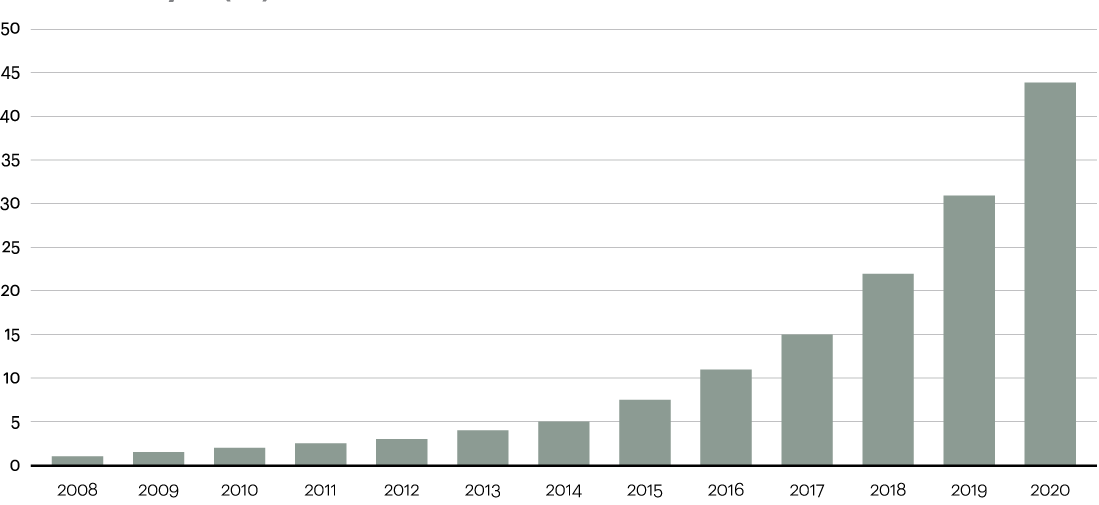
\includegraphics[width=14cm]{./images/Data.png}
       	\caption{Evolución histórica del número de Zeta Bytes de información almacenados y predicción para los próximos años \cite{zeta-bytes}.} 
       	\label{fig:zeta-bytes}
	 \end{figure}

	En resumen, a pesar de la evolución de los computadores en todas sus facetas, la cantidad de datos e información a procesar y almacenar crece incluso a mayor velocidad. Por ejemplo, encontramos empresas como Facebook y Google cuyos usuarios generan una gran cantidad de datos diariamente. Estos datos deben ser tratados en tiempo real para poder mantener los sistemas de recomendaciones asociados. En estos casos se requieren servidores de altas prestaciones para poder tratar tal cantidad de datos en un tiempo razonable. Estos conjuntos de datos adquieren el calificativo ``masivos''. El desarrollo de nuevas tecnologías, algoritmos y herramientas para tratar de forma eficiente conjuntos de datos masivos es lo que se conoce como Big Data \cite{big-data-herrera}.
	
	En este trabajo presentamos una introducción a Big Data y a varias herramientas software existentes, destacando el papel de la ingeniería de servidores en este contexto. En particular, incidimos en la importancia del desarrollo de nuevos benchmarks que permitan evaluar las tecnologías de Big Data de forma clara y objetiva.

	El resto del texto se organiza como sigue. La Sección \ref{sec:big-data} contiene una descripción del concepto de Big Data. En la Sección \ref{sec:mr-hadoop} introducimos el paradigma de programación distribuida Map Reduce y una de las tecnologías libres que lo implementa, denominada Hadoop. En la Sección \ref{sec:tpcx-hs} explicamos uno de los benchmarks existentes para las tecnologías Big Data, denominado TPCx-HS. Por último, en la Sección \ref{sec:conclusion} presentamos las conclusiones obtenidas.

\section{Big Data} \label{sec:big-data}
	
	En esta sección profundizamos en el concepto de big data y en su relación con la ingeniería de servidores. En primer lugar, en la Sección \ref{sec:big-data:que-es} describimos qué es Big Data y qué tipos de problemas involucra. Además, destacamos la importancia de Big Data en el ámbito empresarial y científico. Por último, en la Sección \ref{sec:big-data:ise} mostramos que la ingeniería de servidores es esencial en Big Data debido al uso de la computación de altas prestaciones para el tratamiento de conjuntos de datos masivos.

	\subsection{¿Qué es Big Data?} \label{sec:big-data:que-es}
	
		En la Sección \ref{sec:introduction} hemos incidido en la rápida evolución que han sufrido los computadores. Sin embargo, en muchas aplicaciones encontramos conjuntos de datos que ponen a prueba a los ordenadores más potentes. Estos conjuntos de datos se denominan masivos. El tratamiento de datos masivos tiene dos problemas claros. El primero de ellos es la memoria. Necesitamos computadores con suficiente memoria principal para procesar de forma eficiente un gran flujo de datos. El segundo problema es la capacidad de cómputo necesaria para aplicar algoritmos sobre estos conjuntos de datos. 
		
		Big Data engloba el tratamiento de datos masivos desde el punto de vista tecnológico y algorítmico. En palabras de Michael J. Franklin, profesor de informática en la universidad de Berkley \cite{bd-definition}:
		
		\textit{``Un problema sobre datos entra en el ámbito de Big Data cuando la aplicación de las actuales tecnologías no permite al usuario obtener soluciones  rápidas, efectivas en costo y de calidad''}
	
		Por tanto, Big Data es un concepto relativo a la situación tecnológica de la sociedad. Lo que hoy es Big Data puede no serlo dentro de varios años. Esto asegura que Big Data será un tema recurrente de la literatura especializada. La resolución de problemas de Big Data no cierra su desarrollo sino que abre nuevos retos, siempre habrá un conjunto de datos lo suficientemente grande como para poner a prueba los últimos logros del estado del arte.
	
		Los problemas que entran en el ámbito de Big Data surgen de manera natural en el mundo actual. En palabras de Francisco Herrera triguero, investigador de la Universidad de Granada  \cite{big-data-herrera}:
		
		\textit{``Vivimos en la era de la información. El progreso y la innovación no se ve obstaculizado por la capacidad de recopilar datos sino por la capacidad de gestionar, analizar, sintetizar y descubrir el conocimiento subyacente en dichos datos. Este es el reto de las tecnologías de Big Data.''}
		
		A veces se utiliza el término Big Data para referirse meramente a conjuntos de datos masivos. Sin embargo, los problemas de Big Data constan de múltiples características que los hacen todavía más complejos. En la literatura especializada estas características se denominan las 3 V's de Big Data \cite{big-data}:
	
		\begin{itemize}
			\item \textbf{Volumen.} El tamaño de los conjuntos de datos a procesar es cada vez mayor, por ejemplo, facebook procesa cada día 500 TB de información. Este volumen de datos requiere tecnologías específicas para que los servidores de altas prestaciones puedan manejar la información con éxito.
			\item \textbf{Velocidad.} Necesitamos herramientas que permitan procesar y analizar conjuntos de datos masivos en poco tiempo. Además, es habitual que el procesamiento de los datos deba ser incluso en tiempo real, esto es, los datos llegan al sistema de forma continua y este debe agregar la información de los mismos.
			\item \textbf{Variedad.} Los datos a tratar provienen de una gran variedad de fuentes. Por tanto, las herramientas Big Data deben permitir procesar a la vez datos de diferentes características y tamaños. Es más, habitualmente encontramos datos de tres tipos: estructurados, semi estructurados y sin estructurar. Los datos estructurados son sencillos de clasificar. Sin embargo, los datos sin estructurar son aleatorios y difíciles de analizar. Por su parte, los datos semi estructurados requieren técnicas avanzadas para poder clasificarlos correctamente.
		\end{itemize}
	
		Algunos autores han extendido estas características hasta utilizar un total de 9 V's: veracidad, valor, viabilidad y visualización entre otras \cite{understanding-big-data}. De esta forma se destacan diferentes aspectos del tratamiento de conjuntos de datos masivos como mantener y analizar la veracidad de los datos y poner en valor el conocimiento subyacente.
	
		El término Big Data ha tomado peso en el ámbito empresarial. Actualmente forma parte del área de conocimiento que se denomina inteligencia de negocio (business intelligence) \cite{business-intelligence}. La inteligencia de negocio cubre aquellos problemas relacionados con datos que se resuelven en organizaciones empresariales. Las empresas almacenan información de sus clientes y de toda la actividad realizada. Esta información contiene conocimiento que es valioso para determinar nuevas estrategias de negocio. Podemos decir que el análisis de datos es crucial para que las decisiones tomadas en la empresa sean efectivas. 
	
		Big Data también se considera parte del área denominada ciencia de datos \cite{data-science}. Esta es una temática emergente que aglutina todas las áreas científicas que se encargan del tratamiento de los datos y de la extracción de conocimiento de los mismos. En este contexto, algunos autores denominan Big Data Analytics a la aplicación de Big Data al análisis de datos \cite{big-data-trends}. La ciencia de datos y la inteligencia de negocio están muy relacionadas, siendo el último término más popular en el ámbito empresarial. La importancia de estas áreas de conocimiento ha dado lugar a una nueva profesión, el científico de datos, que es considerada una de las profesiones más valoradas del siglo XXI \cite{data-scientist}.
		
		Cuando uno se enfrenta a un problema de Big Data necesita estudiar y desarrollar tecnologías que permitan el procesamiento de gran cantidades de datos de forma eficiente. Además, debe adaptar los algoritmos que pretenda utilizar a este nuevo ámbito, reduciendo en medida de lo posible complejidad algorítmica de los mismos. La dificultad de este proceso resolutivo es lo que hace que los expertos en Big Data sean muy valorados en el ámbito científico y empresarial. En el resto del documento presentaremos varias tecnologías que se utilizan de forma habitual en Big Data (Hadoop, Spark y Flink) así como un benchmark para Hadoop, denominado TPCx-HS.
		
	\subsection{Ingeniería de servidores en Big Data: computación de altas prestaciones} \label{sec:big-data:ise}
	
		En la Sección \ref{sec:big-data:que-es} destacábamos dos problemas del tratamiento de conjuntos de datos masivos: el conjunto de datos puede no caber en memoria principal y se necesita una gran capacidad de cómputo para ejecutar algoritmos sobre este. La solución a este problema suele ser la aplicación de la computación de altas prestaciones \cite{hpc}.
		
		El término computación de altas prestaciones se refiere a la agregación de varios computadores con el fin de obtener una mayor potencia y rendimiento. Cada uno de los computadores utilizados se denomina nodo mientras que al conjunto de todos los nodos se le llama clúster o servidor de altas prestaciones. La agregación de la capacidad de cómputo de los nodos se consigue gracias a la paralelización y programación distribuida. Todos los nodos realizan tareas simultáneamente que ayudan a la resolución de un problema. El conjunto de todas las tareas a realizar conforma el algoritmo que se ejecuta en el servidor. De esta forma el trabajo a realizar se reparte entre los nodos, obteniendo un menor tiempo de ejecución.
		
		
		Sin embargo, el uso de la computación de altas prestaciones no soluciona de forma directa el problema. Supóngase que una empresa compra un servidor en el cual ejecuta un algoritmo distribuido con eficiencia $\theta(n^2)$ sobre conjuntos de datos masivos. En el momento en el que se compra el hardware consiguen ejecutar el algoritmo en 8 horas, obteniendo resultados en el mismo día. Sin embargo, siguiendo la tendencia mostrada en la Figura \ref{fig:zeta-bytes}, es probable que el conjunto de datos a utilizar se duplique en tamaño dentro de un año. En tal caso el servidor puede tener problemas desde el punto de vista de la memoria y el flujo de dato debido a los cuellos de botella que pueda mostrar el hardware. Por otro lado, aunque no hubiese problemas con la memoria, el algoritmo tardará como mínimo 4 veces más en ejecutarse al tener complejidad cuadrática. Por tanto, la ejecución pasará a durar 32 horas, no pudiendo obtener resultados en un mismo día. 
				
		El ejemplo anterior muestra un problema de escalabilidad inherente a Big Data. Aunque está claro que el procesamiento distribuido en servidores de altas prestaciones es la solución, el crecimiento de los conjuntos de datos hace que el hardware se quede obsoleto en poco tiempo. Una solución puede ser actualizarlo cada año. Sin embargo, una empresa no puede permitirse renovar el hardware anualmente pues esto supondría un aumento de costes, consumo eléctrico, mantenimiento y, además, requiere una gran cantidad de espacio. Consecuentemente, el buen aprovechamiento de los recursos del servidor es necesario para obtener resultados satisfactorios en Big Data. Necesitamos comprar desde un inicio aquel servidor que proporcione el mayor rendimiento para el manejo de datos de manera que la inversión sea rentable a largo plazo. La ingeniería de servidores es clave en esta cuestión.
		
		Por último, hay que destacar que los servidores a utilizar contendrán ingentes cantidades de información de vital importancia. Por tanto, se necesita almacenar los datos en un sistema de archivos tolerante a errores. Esto es, si un nodo o disco duro del servidor se estropea, no se pueden perder datos ni provocar una caída del servidor. En esta situación se encontró Google a principios de este siglo cuando desarrolló Google File System, GFS, que fue presentado oficialmente en 2003 \cite{gfs}. Este es un sistema de archivos escalable y distribuido que utilizan para aplicaciones distribuidas que requieran conjuntos de datos masivos. El sistema proporciona tolerancia ante fallos de forma automática y administra de forma eficiente grandes conjuntos de datos en el servidor, no necesitando que este sea especialmente caro. Además, proporciona escalabilidad en el sentido de que se pueden añadir o eliminar nodos o discos duros sin problemas. De esta forma, se consigue un correcto almacenamiento de los datos en el servidor.
				
		Google File System es un software privado. Basándose en las ideas de este, la fundación Apache ha desarrollado HDFS (Hadoop Distributed File System) \cite{hdfs}. Incidiremos en este en la Sección \ref{sec:mr-hadoop:hadoop}, pues una herramienta esencial dentro de Hadoop.
				
	
%-----------------------------------------------------------------------------------------------------
%	SECCIÓN 2
%-----------------------------------------------------------------------------------------------------

\section{Map Reduce. Hadoop} \label{sec:mr-hadoop}

	En esta sección introducimos Map Reduce, un nuevo paradigma de programación distribuida que es básico en el ámbito de Big Data. En la Sección \ref{sec:mr-hadoop:map-reduce} explicamos el paradigma mientras que en la Sección \ref{sec:mr-hadoop:hadoop} destacamos uno de los softwares libres que lo implementan.

	\subsection{Map Reduce} \label{sec:mr-hadoop:map-reduce}

		En la Sección \ref{sec:big-data:ise} destacábamos el papel central de los servidores de altas prestaciones y la programación distribuida en Big Data. Por tanto, la implementación de algoritmos para Big Data requiere herramientas y librerías que permitan realizar implementaciones distribuidas. Las librerías OPEN MP y MPI son muy conocidas \cite{openmpmpi, openmp}. OPEN MP permite paralelizar cálculos vectoriales. Por su parte, MPI se basa en el paso de mensajes entre hebras como mecanismo para realizar implementaciones distribuidas. Estas librerías operan a bajo nivel y funcionan principalmente con lenguajes de programación como c y c++. 
		
		La implementación de un algoritmo distribuido utilizando estas librerías es muy costosa. El programador debe indicar expresamente el tratamiento distribuido de los datos y cómo se paralelizan los cómputos. Además, tiene que crear las hebras asociadas y encargarse de que el sistema funcione correctamente. Nótese que si durante la ejecución del algoritmo un nodo se estropea, entonces la implementación puede dejar de funcionar a no ser que el programador le haya dedicado mucho tiempo para conseguir que sea tolerante ante fallos. Es más, si uno implementa varios algoritmos distribuidos esencialmente se está implementando el mismo tipo de paralelización una y otra vez.
	
		Recordemos en este punto el problema de escalabilidad de Big Data, destacado en la Sección \ref{sec:big-data:ise}. Es claro que una solución a este problema consiste en reformular los algoritmos a utilizar, mejorando la eficiencia y escalabilidad. Sin embargo, esto implica un gran trabajo de implementación dada la dificultad de la programación distribuida. Ante esta situación en Google se dieron cuenta de la necesidad de desarrollar un nuevo paradigma de programación distribuida. Este debía proporcionar una interfaz que permitiese al programador implementar algoritmos distribuidos de forma simple y eficiente sin tener que centrarse en cuestiones de bajo nivel. La distribución de los datos en los nodos y la tolerancia ante los fallos serían llevadas a cabo por el propio lenguaje de programación de manera que el programador solamente tiene que desarrollar el algoritmo en cuestión. Gracias a esta idea surge el paradigma de programación Map Reduce, que Google hizo público en 2004 \cite{map-reduce1, map-reduce2, map-reduce3}.
	
		Map Reduce se basa en un proceso de abstracción a la hora de implementar algoritmos distribuidos. Los creadores de este paradigma se inspiraron en las funciones map y reduce que suelen estar presentes como primitivas en múltiples lenguajes de programación funcional. En primer lugar, la entrada y la salida de un algoritmo se conciben como dos listas de parejas (clave,valor), que pueden tener tipos distintos. El programador debe proporcionar el código de las funciones map y reduce. Estas funciones se ejecutarán en paralelo en los diferentes nodos del clúster.
		
		\begin{itemize}
			\item La función \textbf{map} toma como entrada una pareja (clave, valor) y produce un nuevo conjunto de parejas (clave, valor), denominado conjunto intermedio. La función map se aplica en paralelo a cada una de las parejas que conforman la entrada del algoritmo. Tras la ejecución de todos los maps, el sistema ordena y filtra los conjuntos intermedios de parejas de manera que a cada posible clave se le asigna una lista con todos los valores que tenía asociados como pareja.
			\item La función \textbf{reduce} toma una clave y una lista de valores asociados a la clave. Se aplica a cada una de las salidas que se han obtenido tras la ordenación y el filtrado de los resultados de los maps. Los valores de cada clave se mezclan mediante el procedimiento indicado por el programador. Este debe devolver al final cero o más parejas formadas por la clave y cada uno de los valores obtenidos tras la mezcla. La lista de valores que se proporciona como argumento a reduce se representa en la implementación mediante un iterador. De esta forma se puede trabajar con listas de valores tan grandes que no quepan en memoria principal.
		\end{itemize}  
		
		Para ejemplificar el funcionamiento de Map Reduce mostraremos un algoritmo distribuido que cuenta el número de ocurrencias de cada una de las palabras de un documento. El Algoritmo \ref{alg:map-reduce} contiene el pseudo-código de este. La función map toma como parámetros el nombre del documento y una string con parte del texto asociado. Por cada palabra que encuentra emite una pareja con la palabra y un 1. La función reduce suma todas las ocurrencias encontradas de la palabra, devolviendo la pareja (palabra, número total de ocurrencias).
		
		\begin{algorithm}
			\caption{Obtención del número de ocurrencias de cada una de las palabras de un texto mediante Map Reduce.}
			\label{alg:map-reduce}

			\begin{subalgorithm}{.4\textwidth}
			\begin{algorithmic}
				\State $key$: Nombre del documento
				\State $value$: Texto del documento
				\Function{map}{String $key$, String $value$}
					\For{each word $w$ in $value$}
						\State EmitIntermediate($w$, \texttt{"}$1$\texttt{"} )
					\EndFor
				\EndFunction
			\end{algorithmic}
			\end{subalgorithm}
			\begin{subalgorithm}{.6\textwidth}
			\begin{algorithmic}
				\State $key$: Palabra
				\State $values$: Conjunto con las ocurrencias de la palabra
				\Function{reduce}{String $key$, Iterator $values$}
					\State $result = 0$
					\For{each value $v$ in  $values$}
						\State $result$ += Int($v$);
					\EndFor
					\State \textbf{return} $key$, String($result$);
				\EndFunction
			\end{algorithmic}
			\end{subalgorithm}
		\end{algorithm}

		La paralelización  la lleva  cabo el sistema de forma automática. Para ello la entrada debe particionarse en $M$ bloques en tiempo de ejecución. Cada uno de estos bloques contiene una lista de parejas (clave, valor). Map Reduce repartirá los bloques en distintos nodos del servidor de forma que cada uno de estos nodos ejecuta la función map sobre cada una de las parejas de su bloque. Las hebras que realizan esta acción se denomina mappers. El programador debe indicar tanto el número de bloques a utilizar ($M$) como definir la función utilizada para el particionamiento de la entrada. Habitualmente se recomienda que cada uno de los $M$ bloques contenga entre $16$ y $64$ MB. 
		
		Conforme los maps terminan de ejecutarse se va realizando la fase de ordenación y filtrado de los resultados. En este ejemplo para cada palabra se obtiene una lista de unos con tantos elementos como el número de veces que se haya encontrado la palabra. Una vez han finalizado los mappers, se pueden ejecutar las hebras que aplican la función reduce. Estas se denominan reducers. Para ello el conjunto de claves intermedias se particiona en $R$ bloques. Cada uno de esto $R$ bloques se asigna a un nodo con un reducer, que ejecutará la función reduce sobre las parejas (clave, iterador) que le correspondan. El programador debe decidir el valor $R$ para obtener el mejor rendimiento posible del sistema. Tras la ejecución de los reduce se obtiene la lista de las palabras encontradas y el número de ocurrencias de las mismas.  La Figura \ref{fig:map-reduce} muestra de forma gráfica este proceso.

		\begin{figure}[H]
			\centering
			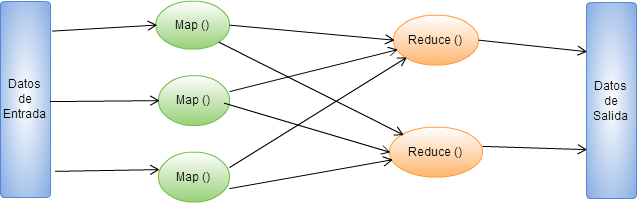
\includegraphics[width=14cm]{./images/MapReduce.png}
			\caption{Aplicación de Map Reduce sobre un conjunto de datos.} 
			\label{fig:map-reduce}
		\end{figure}

		La implementación de Map Reduce se lleva a cabo siguiendo el paradigma maestro - esclavo. La Figura \ref{fig:map-reduce:master-workers} (véase el anexo) muestra el proceso que se realiza de forma interna en una ejecución de Map Reduce con $M=3$ y $R=2$. El primer paso es el particionamiento de la entrada. Tras realizarse este se crea una hebra denominada maestro que se encarga de controlar toda la ejecución. Además, se lanzan tantas hebras como tareas haya que realizar, en total $M+R$. Estas hebras se llaman esclavos y son de dos tipos: mappers y reducers. Los esclavos se almacenan en una cola en la que tienen prioridad los mappers.
		
		Las hebras de la cola se van asignando a los nodos del sistema y los mappers comienzan a ejecutarse. Cada mapper genera parejas intermedias que se almacenan en un buffer de la memoria. Periódicamente, el buffer se vacía, escribiendo las parejas en un disco duro asociado al mapper. En cada disco duro se utilizan $R$ regiones, numeradas desde el $0$ al $R-1$. Las parejas se reparten entre estas regiones utilizando una función hash sobre las claves. De esta manera parejas con la misma clave irán a la misma región disco duro. 

		Como consecuencia, si los datos generados no están uniformemente distribuidos en todas las claves puede suceder que una región contenga mucho más trabajo que otra. A cambio, se obtiene un proceso eficiente para conseguir que todas las parejas con la misma clave vayan a la misma región.
		
		La localización de estas regiones en los discos es enviada al maestro. Cuando un reducer pasa a ejecutarse, el maestro le notifica de la localización de las regiones de los discos que les corresponden (aquellas que tienen el mismo índice que el reducer). Posteriormente, el esclavo llama a los discos para obtener las regiones correspondientes. Nótese que de esta forma todos las parejas con igual clave van al mismo reducer. Tras la obtención de los datos, el reducer los ordena por clave y agrupa aquellos valores que pertenezcan a la misma clave en conjuntos. Si el tamaño de los datos es demasiado grande, entonces una ordenación externa es utilizada.
		
		Cuando todos los mappers se han ejecutado, los reducers comienzan a aplicar la función reduce a sus correspondientes parejas. Cada hebra produce un archivo de salida con los resultados obtenidos. Tras finalizar la ejecución de estas, el control vuelve al usuario. Normalmente se deberían unir los $R$ archivos generados en uno nuevo, para lo cual se requeriría una nueva llamada a MapReduce u otra aplicación distribuida que permita realizar este proceso.

		En este contexto se implementa la tolerancia a errores como sigue. Periódicamente el maestro realiza un ping a cada uno de los esclavos. Si algunos de ellos no le responde, entonces se asume que el nodo ha fallado y se envía su correspondiente trabajo al primer nodo que se encuentre disponible. En caso de que falle un mapper, los reducers son informados de que deben leer los datos de este mapper desde la nueva localización en disco a no ser que ya hayan completado la lectura de los datos de la ejecución errada.

		En definitiva, Map Reduce permite a los programadores con poca experiencia en sistemas distribuidos llevar a cabo implementaciones eficientes para grandes cantidades de datos. De esta manera se ahorra trabajo de implementación, pudiendo dedicarse el programador a mejorar la eficiencia de los algoritmos. Es más, una implementación típica de Map Reduce puede procesar varios tera bytes de datos en servidores con miles de nodos.


	\subsection{Hadoop} \label{sec:mr-hadoop:hadoop}

		La implementación de Google del paradigma de programación Map Reduce es privada. Sin embargo, las publicaciones que hiceron los trabajadores de Google sobre este paradigma han inspirado implementaciones libres de Map Reduce. La más importante sin duda es Hadoop \cite{hadoop-book}. 
		
		Hadoop comenzó a desarrollarse poco después de la publicación de GFS y Map Reduce. Inicialmente el proyecto en cuestión era Apache Nutch \cite{nutch} y tenía como objetivo desarrollar un buscador web libre. El proyecto estaba siendo desarrollado por Doug Cutting entre otros. Sin embargo, el software tenía muchos problemas cuando se ejecutaba sobre un clúster de computadores. Con el fin de solucionar este problema comenzaron a implementar un sistema de archivos distribuidos basado en GFS y una versión de Map Reduce. Este nuevo proyecto pasó a llamarse Hadoop en 2006. Como curiosidad, Hadoop es el nombre del elefante de peluche del hijo de Dough Cutting, que fue director del proyecto.
		
		Hadoop está implementado principalmente en Java, aunque utiliza de forma minoritaria C y utilidades de la línea de comandos. Se encuentra disponible para Windows y los sistemas Unix, aunque solo incluye soporte para Linux. Hadoop incluye 4 módulos básicos \cite{hadoop-doc}:
		 
		\begin{enumerate}
			\item \textbf{Hadoop Common.} Librería con las funciones y utilidades comunes al resto de módulos.
			\item \textbf{Hadoop Distributed File System (HDFS).} Sistema de archivos distribuidos que imita las ideas utilizadas por Google en GFS. Es el núcleo de todas las aplicaciones de Hadoop.
			\item \textbf{Hadoop YARN.} Framework para la asignación de tareas a los nodos y mantenimiento de los recursos un clúster.
			\item \textbf{Hadoop MapReduce.} Implementación del paradigma Map Reduce en el ecosistema Hadoop. Utiliza YARN para procesar en paralelo de grandes conjuntos de datos. Funciona de forma similar a la explicación dada en la Sección \ref{sec:mr-hadoop:map-reduce}. El programador debe proporcionar la implementación de las funciones map y reduce y del módulo de particionamiento de la entrada. Aunque Hadoop está implementado principalmente en Java, permite utilizar Java, Python, Ruby y C++ para programar los algoritmos. Además, Hadoop MapReduce posibilita una alta configuración, como modificar las operaciones de ordenación y filtrado de los datos.
		\end{enumerate}
		
		Además de estos módulos básicos, Hadoop incluye otros subproyectos como Hive, que utiliza Map Reduce para realizar búsquedas SQL sobre los datos almacenados con HDFS, o Spark, que estudiaremos en la Sección \ref{sec:spark-flink}.
		
%-----------------------------------------------------------------------------------------------------
%	SECCIÓN 4
%-----------------------------------------------------------------------------------------------------

\section{Benchmarks: TPCx-HS} \label{sec:tpcx-hs}

	La variedad de computadores es bastante heterogénea. Cada uno realiza de forma eficiente un determinado conjunto de operaciones a consta de presentar peores resultados en otros factores. Por tanto, la comparación entre diferentes modelos de computadores es compleja. Consecuentemente, se han creado benchmarks con el objetivo de aportar elementos de juicio con los que se discernir entre el uso de un computador u otro para una determinada aplicación. Habitualmente el benchmarking se define como la obtención de información útil mediante pruebas empíricas que ayude a una organización a mejorar sus procesos \cite{benchmarking}. Sin embargo, el benchmarking de computadores es un proceso costoso computacionalmente. Gasta tanto energía como mucho tiempo de cómputo. Por tanto, se ha de reservar para cuestiones sean importantes y no para evaluar tareas simples \cite{desv-bench}.
	
	Una técnica utilizada para ver qué sistema nos da más prestaciones son los benchmarks, uno de ellos es TPC. TPC es una organización sin ánimo de lucro que estudia el proceso de transacción y desarrolla benchmarks para bases de datos. El término transacción se suele atribuir a aspectos bancarios. Sin embargo, en este contexto una transacción es un conjunto de operaciones de un computador que incluyen lectura y escritura en disco, llamadas a funciones del sistema operativo, o cualquier forma de transferencia de datos de un sistema a otro. Los benchmarks que produce TPC miden el proceso de transacción y el rendimiento de las bases de datos en términos del número transacciones que se pueden hacer por unidad de tiempo \cite{intro-tpc}.
	
	TPCx-HS (Transaction Processing Performance Council Express Hadoop System) se desarrolló para proveer de una medida del rendimiento fiable, rendimiento relación precio, disponibilidad y, opcionalmente, datos de consumo de energía de los sistemas de Big Data que usen Hadoop. TPCx-HS fue el primer benchmark objetivo que permitía medir tanto hardware como software, como el Hadoop Runtime. \cite{info-tpc}
	
	\subsection{Carga de trabajo de TPCx-HS}
	
		La carga de trabajo de TPCx-HS consiste en los siguientes módulos \cite{tpcxhs}:
		
		\begin{itemize}
			\item HSGen: es un programa que genera los datos según factor de escala, que suele estar entre un 1TB y 10000TB (se denota TB como terabytes).
			\item HSDataCheck: es un programa que comprueba el cumplimiento del conjunto de datos.
			\item HSSort: es un programa que ordena los datos según un orden total.
			\item HSValidate: es un programa que valida la salida, es decir, los resultados obtenidos.
		\end{itemize}
	
	\subsection{Fases de ejecución del benchmark}
		Una ejecución válida consiste en cinco fases separadas que corren secuencialmente. Estas fases no se solapan en su ejecución, es decir, el comienzo de la fase 2 no puede darse hasta que la fase 1 esté completa. Para que comience cada fase se necesita de un script llamado $<TPCx-HS-master>$ que es el que inicia cada fase y que puede ser ejecutado desde cualquier nodo del sistema que se está bajo test \cite{tpcxhs}.
		
		Una ejecución válida consiste en cinco fases separadas que corren secuencialmente. Estas fases no se solapan en su ejecución, es decir, el comienzo de la fase 2 no puede darse hasta que la fase 1 esté completa. Para que comience cada fase se necesita de un script llamado <TPCx-HS-master> que es el que inicia cada fase y que puede ser ejecutado desde cualquier nodo del sistema que esté bajo el test \cite{tpcxhs}.

		
		Las fases de ejecución son las siguientes:
		
		\begin{itemize}
			\item Fase 1: se generan los datos de entrada usando HSGen. Se han de copiar en un soporte duradero y hacer la copia replicada en tres discos (llamado \textit{"3-ways replication"}), que suelen ser el principal, el secundario y uno de respaldo \cite{replication}.
			\item Fase 2: se verifica la validez del conjunto de datos usando HSDataCheck. El programa sirve para verificar la cardinalidad, tamaño y el factor de réplica de los datos generados. Si el programa reporta un fallo, entonces la ejecución no es válida y se deberá volver a empezar.
			\item Fase 3: se lanza el programa HSSort con el que se ordena los datos de entrada. Esta fase muestra los datos de entrada y los datos de salida (los datos ya ordenados). Al igual que en la fase 1, se han de copiar los datos en un soportde duradero y hacer el \textit{"3-ways replication"}.
			\item Fase 4: se comprueba la viabilidad del conjunto de datos usando HSDataCheck. El programa comprueba la cardinalidad de los datos, tamaño y el factor de replicación de los datos ordenados. Si el programa reporta un fallo, entonces la ejecución no es válida y se deberá volver a empezar.
			\item Fase 5: una vez que en la fase 4 se ha comprobado la cardinalidad de los datos antes y después de ordenarlos, se procede a la validación de los datos con HSValidate. Como su nombre indica, HSValidate comprueba que los datos de salida sean correctos, es decir, se realiza la verificación de la replicación de los datos. Si reporta el fallo consisten en que el HSSort no generó el correcto orden de salida, la ejecución se considerará inválida.
		\end{itemize}
		
		El benchmark consiste en dos ejecuciones (ver la Figura \ref{fig:ejecucionesTPC}) y cada vez que se ejecuta una fase se ha de especificar el tiempo que ha llevado la ejecución. Entre la primera ejecución de las cinco fases y la segunda, hay una fase intermedia que sirve para limpiar el sistema, conocida como \textit{"file system cleanup"} y, lógicamente, no se permite ninguna actividad durante dicha fase. Una vez realizadas las dos ejecuciones se obtiene el tiempo total de ejecución que servirá para calcular datos en la fase de medición.
		
		\begin{figure}[h]
			\centering
			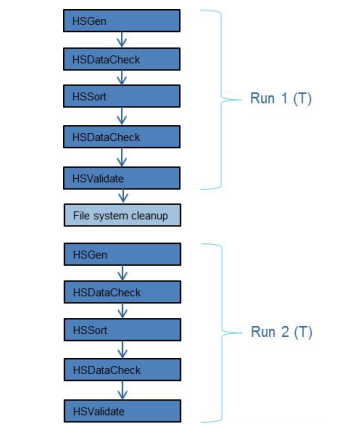
\includegraphics[width=5cm]{./images/executionsTPC.png}
			\caption{Gráfico de las ejecuciones de TPCx-HS} 
			\label{fig:ejecucionesTPC}
		\end{figure}
		
		Como consideraciones finales en la ejecución, el sistema bajo test no puede ser reconfigurado o cambiado durante o entre cualquiera de las fases de la ejecución ni tampoco entre la primera y la segunda ejecución. Cualquier cambio que se haga en el sistema se deberá realizar antes del comienzo de la fase 1 de la primera ejecución. El factor de escala usado en el conjunto de datos del test debe ser escogido del conjunto de factores de escala definido como sigue: 1TB, 3TB, 10TB, 30TB, 100TB, 300TB, 1000TB, 3000TB, 10000TB.
	
	\subsection{Medida del rendimiento}
	
		Para hacer el análisis de la medida del rendimiento, TPCx-HS define las siguientes medidas:
		
		\begin{itemize}
			\item HSph@SF: refleja la medida del rendimiento de TPCx-HS.
			\item \$/HSph@SF: es la medida del rendimiento-precio.
			\item Si se escoge la opción de \textit{"TPC-energy"}, la medida de la energía que hace TPCx-HS informa de la potencia por rendimiento. \\
		\end{itemize}
		
		La medida del rendimiento se representa con HSph@SF, que se mide con la siguiente expresión:
		
		$$ HSph@SF = \frac{SF}{T/3600} $$
		
		donde:
		\begin{itemize}
			\item SF es el factor de escala escogido.
			\item T es el tiempo total que se obtuvo al sumar el tiempo de las dos ejecuciones. \\
		\end{itemize}	
		
		La medida del rendimiento-precio se puede calcular con la siguiente fórmula. Dicha medida usa una lógica negativa ya que a menor valor se tiene un mejor rendimiento-precio.
		
		$$ \$/HSph@SF = \frac{P}{HSph@SF} $$
		
		donde P es el costo del sistema en el que se han hecho las ejecuciones.
		
		
		\subsection{Comparación de la medida}
		
		Un resultado dado por la ejecución de TPCx-HS sólo puede ser comparado con otro resultado que provenga de la ejecución de este benchmark y que tenga el mismo factor de escala. Otras consideraciones a tener en cuenta son:
		
		\begin{itemize}
			\item Los resultados producidos por test que tienen diferente factor de escala no son comparables, debido a los \textit{retos} computacionales encontrados en volúmenes de datos de distinto tamaño.
			\item Si los resultados medidos con diferentes factores de escalas aparecen impresos o en algún documento electrónico, entonces cada referencia que se haga a uno de estos resultados se ha de especificar claramente el factor de escala que se usó para obtener esos resultados. Si los resultados aparecen de forma gráfica, el factor de escala en el que se basó dicha medición se deberá poder discernir, por ejemplo usando una etiqueta en uno de los ejes.
		\end{itemize}
		
		
		La figura \ref{fig:ejemplo} (véase el anexo) presenta una tabla con los resultados para algunas compañías donde se puede ver el factor de escala usado, el sistema y los resultados obtenidos tras la ejecución del benchmark.

%-----------------------------------------------------------------------------------------------------
%	SECCIÓN 5: CONCLUSIÓN
%-----------------------------------------------------------------------------------------------------

\section{Conclusión} \label{sec:conclusion}

	Podemos decir que Big Data es un área que aúna tanto la ingeniería del software como la ingeniería de servidores y la ciencia de datos.

%-----------------------------------------------------------------------------------------------------
%	SECCIÓN 6: REFERENCIAS
%-----------------------------------------------------------------------------------------------------

\printbibliography

%-----------------------------------------------------------------------------------------------------
%	SECCIÓN 7: ANEXO
%-----------------------------------------------------------------------------------------------------

\section*{Anexo}

	\begin{figure}[H]
		\centering
		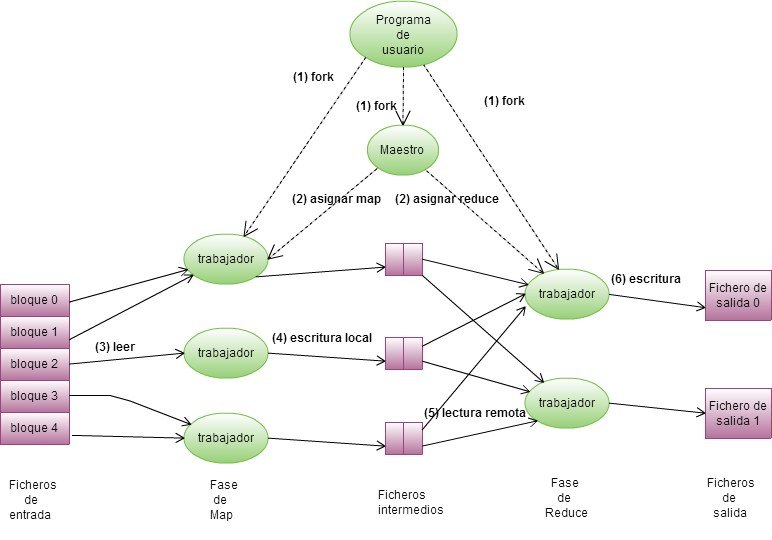
\includegraphics[width=14cm]{./images/MapReduce-MasterWorkers.png}
		\caption{Funcionamiento interno de Map Reduce.} 
		\label{fig:map-reduce:master-workers}
	\end{figure}

			
	\begin{figure}[H]
		\centering
		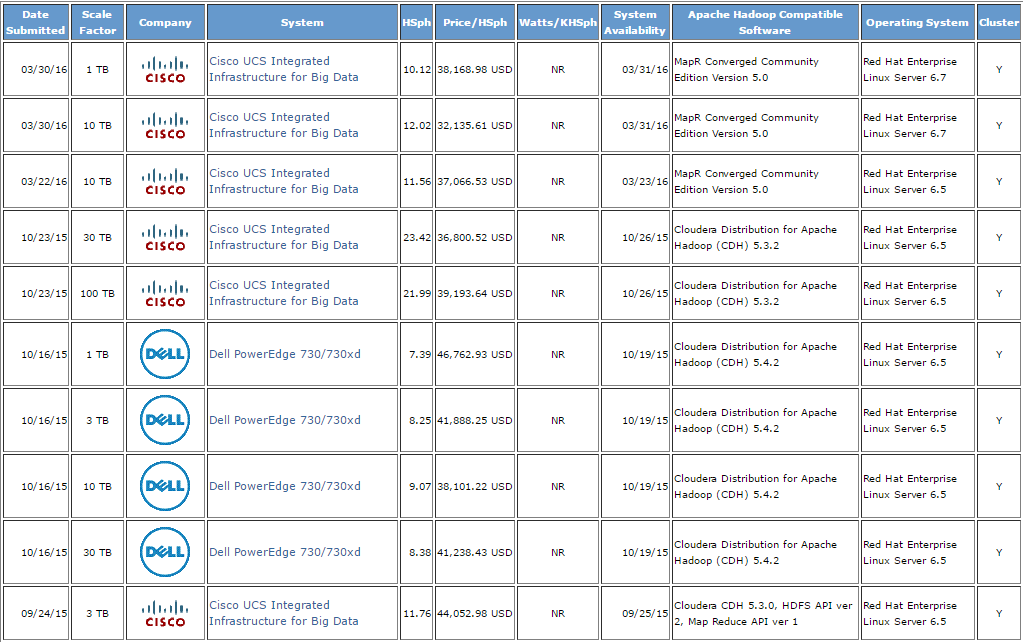
\includegraphics[width=15cm]{./images/examples.png}
		\caption{Tabla de resultados obtenidos con TPCx-HS \cite{ejemplos}.} 
		\label{fig:ejemplo}
	\end{figure}
\end{document}